\documentclass[a4paper,12pt]{article}

\usepackage[utf8]{inputenc}
\usepackage[T1]{polski}
\usepackage{helvet}
\usepackage{graphicx}
\usepackage{color}
\usepackage{xcolor}
\usepackage{listings}
\usepackage{geometry}
\usepackage{caption}
\usepackage{makeidx}
\usepackage{longtable}
\usepackage{multirow}
\usepackage{wrapfig}

\geometry{hmargin={2cm, 2cm}, height=10.0in}
\DeclareCaptionFont{white}{\color{white}}
\DeclareCaptionFormat{listing}{\colorbox{gray}{\parbox{\textwidth}{#1#2#3}}}
\captionsetup[lstlisting]{format=listing,labelfont=white,textfont=white}
\lstset{ %
language=Octave,                % choose the language of the code
basicstyle=\footnotesize,       % the size of the fonts that are used for the code
numbers=left,                   % where to put the line-numbers
numberstyle=\footnotesize,      % the size of the fonts that are used for the line-numbers
stepnumber=1,                   % the step between two line-numbers. If it's 1 each line 
                                % will be numbered
numbersep=5pt,                  % how far the line-numbers are from the code
backgroundcolor=\color{white},  % choose the background color. You must add \usepackage{color}
showspaces=false,               % show spaces adding particular underscores
showstringspaces=false,         % underline spaces within strings
showtabs=false,                 % show tabs within strings adding particular underscores
frame=single,	                % adds a frame around the code
tabsize=2,	                % sets default tabsize to 2 spaces
%captionpos=b,                   % sets the caption-position to bottom
breaklines=true,                % sets automatic line breaking
breakatwhitespace=false,        % sets if automatic breaks should only happen at whitespace
title=\lstname,                 % show the filename of files included with \lstinputlisting;
                                % also try caption instead of title
escapeinside={\%*}{*)},         % if you want to add a comment within your code
morekeywords={*,...}            % if you want to add more keywords to the set
}

\lstloadlanguages{ Perl }

\makeindex

\begin{document}

% =====  STRONA TYTULOWA PRACY INŻYNIERSKIEJ ====
% ostatnia modyfikacja: 2009/07/01, K. Malarz

\thispagestyle{empty}

%% ------------------------ NAGLOWEK STRONY ---------------------------------
\begin{figure}
\vspace{-13cm}
\hspace{-4cm}

\includegraphics[height=29.3cm]{grafika/agh_nzw_a_pl_1w_wbr_cmyk.pdf}\\
\vspace{-13.9cm}
\end{figure}
\rule{26mm}{0pt}
{\large\textsf{Wydział Fizyki i Informatyki Stosowanej}}\\
\rule{\textwidth}{3pt}\\
\rule[2ex]
{\textwidth}{1pt}\\
\vspace{7ex}
\begin{center}
{\bf\LARGE\textsf{Praca inżynierska}}\\
\vspace{13ex}
% --------------------------- IMIE I NAZWISKO -------------------------------
{\bf\Large\textsf{Krystian Wojtas}}\\
\vspace{3ex}
{\sf \small kierunek studiów:} {\bf\small\textsf{informatyka stosowana}}\\
\vspace{1.5ex}
{\sf \small kierunek dyplomowania:} {\bf\small\textsf{metody numeryczne}}\\
\vspace{10ex}
%% ------------------------ TYTUL PRACY --------------------------------------
{\bf\huge\textsf{Kompilator języków klasy LL do wybranego kodu bajtowego}}\\
\vspace{14ex}
%% ------------------------ OPIEKUN PRACY ------------------------------------
{\sf \Large Opiekun:} {\bf\Large\textsf{dr inż. Maciej Wołoszyn}}\\
\vspace{22ex}
\textsf{\bf\large\textsf{Kraków, styczeń 2011}}
\end{center}
%% =====  STRONA TYTUŁOWA PRACY INŻYNIERSKIEJ  ====

\newpage

%% =====  TYŁ STRONY TYTUŁOWEJ PRACY INŻYNIERSKIEJ  ====
{\sf Oświadczam, świadomy odpowiedzialności karnej za poświadczenie nieprawdy, że niniejszą pracę dyplomową wykonałem osobiście i samodzielnie i nie korzystałem ze źródeł innych niż wymienione w pracy.}

\vspace{14ex}

\begin{center}
\begin{tabular}{lr}
~~~~~~~~~~~~~~~~~~~~~~~~~~~~~~~~~~~~~~~~~~~~~~~~~~~~~~~~~~~~~~~~~ &
................................................................. \\
~ & {\sf (czytelny podpis)} \\
\end{tabular}
\end{center}

%% =====  TYL STRONY TYTULOWEJ PRACY INŻYNIERSKIEJ  ====

\newpage
\linespread{1.3}
\selectfont

\noindent
Na kolejnych dwóch stronach proszę dołączyć kolejno recenzje pracy popełnione przez Opiekuna oraz Recenzenta (wydrukowane z systemu MISIO i podpisane przez odpowiednio Opiekuna i Recenzenta pracy). Papierową wersję pracy (zawierającą podpisane recenzje) proszę złożyć w dziekanacie celem rejestracji.

\vspace{85mm}
\newpage
\tableofcontents

\newpage
\section{Wstęp}
Celem pracy jest omówienie zasady działania kompilatora języków o gramatykach klasy LL na przykładzie Pascala oraz praktyczne zaimplementowanie algorytmów skanowania tokenów z wykorzystaniem wyrażeń regularnych, parsowania wraz z konstrukcją drzewa rozbioru syntaktycznego oraz generowania wynikowego kodu bajtowego.

\subsection{VM}
Obecnie oprogramowanie wysokopoziomowe często tworzy się w językach z natury niezależnych od sprzętu oraz systemu operacyjnego, na których jest ono uruchamiane. W jaki sposób jest to realizowane? Otóż kod napisany przez programistę przetwarzany jest w procesie zwanym kompilacją do postaci kodu pośredniego - bajtkodu. Bajtkod jest całkiem bliski asemblerowi, z tą różnicą że jego procesor nie istnieje w rzeczywistości. Dlatego do uruchomienia potrzebny jest w systemie proces maszyny wirtualnej, która iterpretuje kod pośredni i na tej podstawie zadaje procesorowi odpowiednie instrukcje kodu maszynowego. Maszyna wirtualna przejmuje na siebie obowiązki zarządzania dostępnymi rejestrami i pamięcią. 

Jak widać VM zapewnia warstwę abstrakcji, która unifikuje różnorodność architektur komputerowych i systemów operacyjnych. To właśnie gwarantuje przenośność pisanego wysokopoziomowego kodu.

\subsection{Założenia}
Projekt z założenia ma czytać dowolny język, jeśli spełnia on warunki gramatyki klasy LL. Definicja języka zapisana jest w zewnętrznym pliku. Projekt może też generować dowolny bytecode. Aby to osiągnąć i umożliwić wykorzystanie pełnej optymalizacji, nawet dla najbardziej kuriozalnych konstrukcji opcodów, do syntezy wykorzystuje się klasę abstrakcyjną. Zgodnie ze wzorcem projektowym Inverse of Control w czasie przetwarzania źródeł wywołuje się na niej odpowiednie metody. Ukonkretyzowanie tej klasy powoduje generowanie dowolnego kodu pośredniego.

\newpage
\section{Perl}
Autorem języka jest Larry Wall, zaczął nad nim pracę w 1987r. Dokładnie 18 grudnia udostępnił pierwsza maszynę wirtualną na grupie dyskusyjnej comp.sources.misc. Przez następne lata język gwałtownie się rozwijał. Zyskał sobie rzesze zwolenników ze względu zarówno na zwinność integracji potężnej mocy drzemiącej w konstrukcjach wyrażeń regularnych jak i łatwość implementacji złożonych struktur danych. Funkcjonalny kod powstaje szybko i przyjemnie. W projekcie używałem wersji
\begin{verbatim}
$perl -version
This is perl 5, version 12, subversion 2 (v5.12.2) built for i686-linux-multi
\end{verbatim}
\begin{figure}[h!]
  \centering
    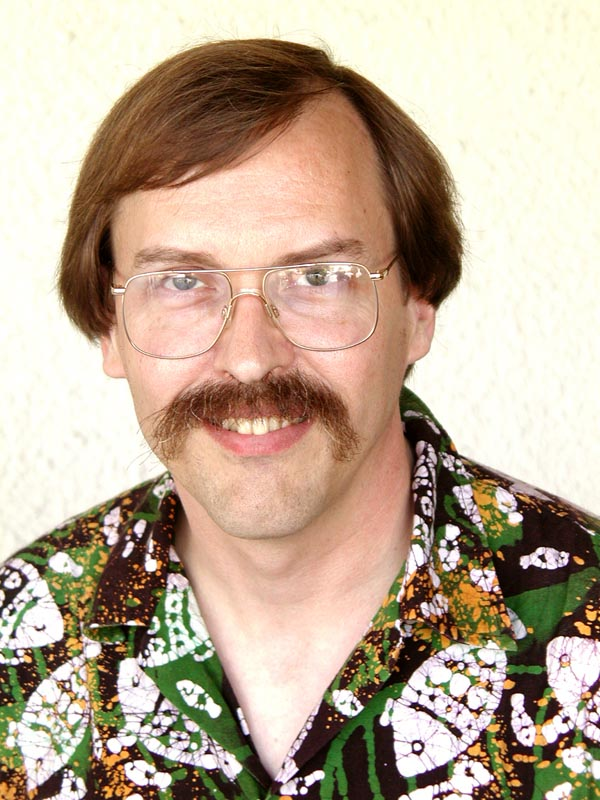
\includegraphics[width=0.5\textwidth]{grafika/larry_wall.jpg}
  \caption{Larry Wall, twórca języka}
\end{figure}

\newpage
\subsection{Dynamiczna VM}
Najciekawszą cechą maszyny wirtualnej Perla jest dynamika. Może ona zmieniać swoje zachowanie w czasie kompilacji po załadowaniu projektowanych ku temu modułów. Przykładowo w Perlu de facto nie występuje konstrukcja switch znana z innych języków programowania
\begin{verbatim}
switch(liczbaCalkowita) {
  case 0:
    print("Wybrano 0");
    break;
  case 1:
    ..
  default
    ..
}
\end{verbatim}
Jednakże po użyciu modułu switch\footnote{http://www.misc-perl-info.com/perl-switch.html inne sposoby konstrukcji switcha} dostępna staje się konstrukcja
\begin{verbatim}
use feature "switch";
given($literalZnakowy) {
  when(/regExp1/) {
    print("Literal pasuje do wyrazenia 1");
  }
  default {
    print("Zachowanie domyslne");
  }
}
\end{verbatim}
Jest to switch z tą różnicą, że \verb|$literalZnakowy| jest badany pod kątem pasujących wyrażeń regularnych, a więc jest znacznie potężniejszy.

% *todo oficjalnie delegacja znana w kregach inzynierii oprogramowania

\subsection{Referencje}
Ogromną zaletą jest łatwość tworzenia i operowania złożonymi strukturami danych. Są trzy podstawowe typy zmiennych: skalar będący liczbą całkowita, literałem znakowym bądź wskaźnikiem, oraz tablica i hash.

Mając referencję do struktury \verb|$r|, sprawdzamy na jaki typ wskazuje stosując \verb|ref $r|. Znając jej typ wykonamy rzutowanie na skalar \verb|$$r|, tablicę \verb|@$r| lub na hasha \verb|%$r|. Dla zobrazowania idei posłużę się kilkoma przykładami uruchomionymi w debuggerze.
\begin{verbatim}
$ perl -d -e 1

Loading DB routines from perl5db.pl version 1.33
Editor support available.

Enter h or `h h' for help, or `man perldebug' for more help.

main::(-e:1):	1
  DB<1> $liczba = 3;

  DB<2> $literal = 'drugie'.$liczba;

  DB<3> @tab = ( 1, 'dwa', $liczba, \$literal );

  DB<4> x \@tab
0  ARRAY(0x8edb170)
   0  1
   1  'dwa'
   2  3
   3  SCALAR(0x8edb130)
      -> 'drugie3'
  DB<5> %hash = ( 'atrybut' => 'przykladowy', 'tabP' => \@tab );

  DB<6> $tab2P = [ [ @tab ], \%hash ];

  DB<7> x $tab2P
0  ARRAY(0x8f11d80)
   0  ARRAY(0x8edb010)
      0  1
      1  'dwa'
      2  3
      3  SCALAR(0x8edb130)
         -> 'drugie3'
   1  HASH(0x8edb370)
      'atrybut' => 'przykladowy'
      'tabP' => ARRAY(0x8edb170)
         0  1
         1  'dwa'
         2  3
         3  SCALAR(0x8edb130)
            -> REUSED_ADDRESS

\end{verbatim}
W pierwszych 3 krokach tworzone są zmienne, używam konkatenacji (znak \verb|.|) i dereferencji (znak \verb|\|). Następnie wyświetlam strukturę na podstawie pobranego jej adresu. Tworzę hash oraz zmienną tab2P, którą drukuję. Widać, że wyrażenie \verb|$tab2P[1]->{tabP}| wskazuje przez adres 0x8edb170 na tablice \verb|\@tab|. Natomiast \verb|$tab2P[0]| wskazuję na identyczną tablicę, jednak znajdującą się pod innym adresem. Kopiowanie wykonaliśmy w kroku 6: \verb|[ @tab ]| utworzyło nową, anonimową tablicę o zawartości takiej jak \verb|@tab| i zwróciło do niej referencję, zapisaną właśnie w \verb|$tab2P[0]|.
\subsection{Prawda}
Skalar \verb|$zmienna| jest fałszem gdy jest pusty tj. 0, ''. Ta sama maksyma dotyczy tablic i hashy. A co nie jest fałszem, jest prawdą.
\subsection{OOP}
Mechanizm klas jest dość prymitywny. Procedury grupuje się w pakiety używając słowa package. W tej przestrzeni nazw wywołuje się procedurę pełniącą rolę konstruktora, zazwyczaj new lub create
\begin{verbatim}
use NowyModul;
$nm = NowyModul->new( 'argument' );
\end{verbatim}
Używając strzałki przekazujemy jako pierwszy argument nazwę modułu NowyModul, dopiero kolejnym będzie 'argument'. Zapis jest ekwiwalentny\footnote{my \$nm = new NowyModul( 'argument' ) również wywiera ten sam efekt }
\begin{verbatim}
$nm = NowyModul::new('NowyModul', 'argument');
\end{verbatim}
Znajduje to zastosowanie w konstruktorze
\begin{verbatim}
package NowyModul
sub new {
  $class = shift; # pobiera pierwszy argument czyli nazwe modułu
  $self = {};  # tworzy anonimowy hash i przypisuje do niego referencje
  bless $self, $class; # sztuczka obiektu
  $self->{arg} = shift; # wpis w hashu kolejnego argumentu
  return $self;
}
\end{verbatim}
Trik polega na zmianie typu wskaźnika w linii bless. Funkcja ta wiąże w wewnętrznych strukturach vm nazwę pakietu \verb|$class| tj NowyModul ze strukturą \verb|$self|, tu referencja do hasha. Od tej pory  \verb|$self| jest wciąż tą samą strukturą, jednak tym razem z przypisaną własną przestrzenią nazw. Można więc wołać na niej funkcje zdefiniowane w jej pakiecie. Programista musi zagwarantować że funkcje te będą poprawnie operować stworzoną strukturą, można już powiedzieć, obiektu.

Czym byłoby OOP bez dziedziczenia? Perl wychodzi naprzeciw potrzebom programistów hierarchizacji klas i unikania redundancji pisanego kodu, oczywiście na swój własny sposób. Jeśli wywoływanej funkcji nie znajdzie w danym pakiecie, sprawdza jego publiczną tablicę \verb|@ISA|. Przegląda kolejne jej wpisy nazw modułów i na nich próbuje odpalić brakującą funkcję. \verb|@ISA| każdego napotkanego modułu także jest sprawdzana. Możliwe jest zatem wielodziedziczenie
\begin{verbatim}
our @ISA = qw(KlasaBazowa1 KlasaBazowa2);
\end{verbatim}

\subsection{AOP}
Aspekty są paradygmem programowania. W jego terminologii wywoływanie metody nazywane jest punktem złączenia. Dowolny zestaw punktów złączeń, inaczej dowolnie wybrany zestaw metod, nosi nazwę punktu przecięcia. Punktowi przecięcia można zaserwować tzw. radę, tj. wykonanie dodatkowego kodu w momencie powrotu z punktu złączenia, bezpośrednio przed jego nastąpieniem, w przypadku zwrócenia wartości lub wystąpienia wyjątku. Radą uzyskujemy dostęp do kontekstu wywołania metody dzięki czemu można modyfikować przekazane argumenty, zwracać zupełnie inną wartość.

%implementacja w vm
\lstinputlisting[label=zrodla::aspekty,caption=Przykład użycia aspektów]{zrodla/aspekty.pl}
Wyjście programu:
\begin{verbatim}
1+1=2
2+2=5
\end{verbatim}

Jak to jest zrobione? - chciałoby się rzec przywołując tytuł popularnego programu na kanale Discovery.*hah del*
Adres funkcji przed i po zastosowaniem rad sie nie zmienia. 

Co ciekawe, porównując języki z platformy .Net lub Jave, tam dodatkowe słowa kluczowe nie mogą zostać użyte i aby osiągnąć AOP należy używać dedykowanych kompilatorów z poziomu źródeł lub ponownie przetwarzać kod bajtowy uzupełniając go o brakującą funkcjonalność w punktach złączeń.

\newpage
\section{Kompilator}
W procesie przetwarzania kodu źródłowego programu wyróżniamy główne etapy front, w którym przeprowadza się analizy zadanego kodu, oraz end, w którym produkuje się z zebranych danych kod bajtowy.

%\subsection{Front}
\subsection{Leksyka}
Tekst źródłowy jest serią znaków, należy z nich wydobyć kolejne wzorce jak słowa kluczowe, nazwy, liczby
zmienno- lub stałoprzecinkowe, operatory. Należy znalezionym słowom przyporządkować typ i wrzucać je do kolejki.
\subsubsection{Terminy}
Strumień znaków tekstu źródłowego dzieli się na mniejsze ciągi nazywane leksemami na podstawie znanej klasyfikacji. Klasyfikacja zapewnia przyporządkowanie leksemowi odpowiadającego mu typu - klasy. Każda klasa ma własną nazwę, słowny opis ją wyrażający, reprezentowane wyrażenie regularne i możliwe znaki następujące po leksemie.
\subsubsection{Wymagania}
Stosuje się warunek znaku występującego bezpośrednio po wyrażeniu. Dzięki temu ciąg returnD nie zostanie trafiony przez RETURN, a złapie go NAZWA, czego oczekujemy.

Liczba zmiennoprzecinkowa zawiera w sobie w początkowych znakach liczbę stałoprzecinkową. Aby ją prawidłowo rozpoznać nadaje się leksemom priorytety według kolejności deklaracji w opisie języka.

Należy dopisać również pewne wzorce, które ewidentnie są błędami w kodach źródłowych. NSTR oraz LERROR są tego praktycznymi dowodami. Takie leksemy ujawnią niesiony błąd w kolejnym kroku analizy podczas budowania drzewa rozbioru.

\subsubsection{Opis języka}
Klasyfikacja zawarta jest w pliku opisu języka. Interesujące są pierwsza kolumna ze słowami pisanymi wielkimi literami - nazwa klasy oraz trzy kolumny z wyrażeniami zawartymi pomiędzy czwartym separatorem. Pierwsze takie wyrażenie regularne charakteryzuje leksem, następne wyrażenie wyszczególnia możliwe znaki występujące po nim. Ostatnie wyrażenie stanowi słowny opis co klasa wyraża. Przykładowe wiersze, czwarty separator to \verb|!|
\begin{verbatim}
WHILE	!while!	!\s|,|\.|:|;|\(|\)|\+|-|\*|\/|<|>|=!	!slowo kluczowe: while!
LOGIKA	!true|false!	!\s|\)!	!wyrazenie logiczne!
LZNAKOWY	!"(\w|\s|_|\+|-|\$|~|#|&|@|:)*"!	!!	!literal znakowy!
NSTR	!"[^"\n]*!	!\n!	!NIEZAMKNIETY STRING!
NAZWA	![a-zA-z]\w*!	!\s|,|\.|:|;|\(|\)|{|}|\+|-|\*|\/|<|>|=!	!nazwa wlasna!
LERROR	!([^\s]+)!	!,|\.|:|;|\(|\)|\+|-|\*|\/|<|>|=!	!LEKSYKALNY BLAD!
\end{verbatim}
Słowo kluczowe z klasy \verb|WHILE| pasuje tylko do znalezionych ciągów kolejnych małych liter \verb|while|, a następować po nim może którykolwiek ze znaków \verb|spacja|, \verb|tab|, \verb|,|, \verb|.|, \verb|:|, \verb|;|, \verb|(|, \verb|)|, \verb|+|, \verb|-|, \verb|*|, \verb|/|, \verb|<|, \verb|>|, \verb|=|. Klasa \verb|LOGIKA| żąda słowa \verb|true| lub \verb|false|, po nim biały znak. Dopasowując \verb|LZNAKOWY| wymagamy aby zaczynał i kończył się cudzysłowem, w środku mogą wystąpić litery, cyfry i widoczne dopuszczalne znaki.

Zapis wczytywania klasyfikacji z pliku opisu języka
\begin{verbatim}
if($linia =~
  /^\s*(\w+)[^$t3]*$t3\s*$t4([^$t4]+)$t4\s*$t4([^$t4]*)$t4\s*$t4([^$t4]*)$t4/) {
  
  push @klasyfikacja, {
    produkcja => $1,
    wzorzec => "($2)",
    terminator => "($3)",
    opis => $4
  };
}
\end{verbatim}
\subsubsection{Logika}
Algorytm wyszukiwania leksemów analizuje kolejne linie kodu użytkownika i próbuje odnaleźć w nich każdy ze zdefiniowanych wzorców. Zapamiętuje wzorzec który zaczyna się od najwcześniejszej pozycji w linii. Jeśli kilka wzorców zacznie się od tego samego miejsca, priorytet ma ten, którego definicja jest wcześniejsza. Po wybraniu leksemu, jest on wycinany z linii wraz z białymi znakami go otaczającymi i trafia do kolejki. Linie są analizowane do wyczerpania posiadanych znaków.
\newpage
\lstinputlisting[label=Kompilator::Pascal::Leksyka,caption=główna część metody analizuj z klasy Kompilator::Pascal::Leksyka]{zrodla/leksyka_analizuj.pl}

\subsection{Syntaktyka}
Mamy zestaw słów łącznie z ich typami. Na ich podstawie budowana jest struktura drzewiasta zapisanego programu tzw. drzewo rozbioru syntaktycznego. Efektem ubocznym tej analizy jest zbadanie poprawności użytych słów tzn. wyłapywane są błędy takie jak pozbawiona sensu linia 'var var zmienna var'.
\subsubsection{Terminy}
Tutaj niechybnie spotykamy się z podstawowym pojęciem produkcji. Oznacza ona odzwierciedlenie symbolu w zestaw symboli precyzyjniejszych. Uwarunkowana jest badanym aktualnie leksemem. Symbole są rozwijane do chwili napotkania symbolu terminalowego, w idealnym świecie, oznaczającego aktualny leksem. Wtedy leksem zostaje zawieszony na drzewie i badany zostaje następny w kolejce.
\subsubsection{Gramatyka LL}
%todo Cytaty
Gramatyka LL to taka, w której czytamy słowo podczas sprawdzania od lewej do prawej, oraz taka, że
możemy podjąć podczas wyprowadzenia lewostronnego jednoznaczną decyzję, którą produkcje
wybrać.

Gramatyka LL(1) to gramatyka LL taka, że podczas podejmowania decyzji, którą produkcję wybrać
analizujemy dokładnie jeden symbol słowa.

Dla zobrazowania podam przykład praktyczny z języka C: % TODO (klasa LR) ?
\begin{verbatim}
int a;
int b();
\end{verbatim}
W pierwszej instrukcji zdefiniowaliśmy zmienną \verb|a|, w drugiej funkcję \verb|b|. 
Zatem po napotkaniu słowa \verb|int| nie można stwierdzić, czy czytana instrukcja będzie deklaracją zmiennej czy funkcji.
Inaczej jest w języku Pascal
\begin{verbatim}
var a:integer;
function b(): integer;
\end{verbatim}
W tym przypadku wiemy po pierwszym słowie co dokładnie będzie deklarowane i jakich kolejnych leksemów można się spodziewać. W Pascalu także miejsca deklaracji są ściśle określone. Po drugiej stronie, w C, można deklarować zmienne na każdym poziomie zagnieżdżania bloków.

Mówimy, że parser LL wykonuje parsowanie metodą zstępującą (ang top-dawn) ponieważ z produkcji najwyższego poziomu próbuje dotrzeć do liści.
\subsubsection{Wymagania}
Celem tego etapu jest stworzenie drzewa rozbioru syntaktycznego. Korzeniem drzewa jest byt abstrakcyjny \verb|program| - nieterminal. Kolejnymi gałęziami tego symbolu są
\begin{verbatim}
deklaracjeOpcj proceduryOpcj START instrukcje END
\end{verbatim}
Czy gałąź \verb|deklaracjeOpcj| się rozwinie zależy od przetwarzanego kodu źródłowego. Jeśli zaczyna on się od słowa \verb|proc| to widać, że użytkownik nie deklaruje żadnych zmiennych globalnych, podczepiony tutaj zostanie terminal abstrakcyjny \verb|EPSILON| i rozkład \verb|deklaracjeOpcj| się kończy. Z kolei dla \verb|proceduryOpcj| słowo źródłowe \verb|proc| jest jak najbardziej oczekiwanym słowem i nastąpi rozwój tej gałęzi. Po jego zakończeniu musi wystąpić terminal \verb|START|, czyli słowo kluczowe \verb|start| będzie musiało na tym etapie wystąpić w źródle, inaczej zgłaszany jest błąd kompilacji.

Aby poznać dokładne działanie algorytmu zapoznajmy się z danymi wejściowymi. Są to kolejka leksemów pozyskana w poprzedniej analizie oraz wykreowana na bieżące potrzeby tablica parsingu. Tablica parsingu przyporządkowuje każdej parze aktualnie analizowanego nieterminala i aktualnie badanego leksemu z kolejki źródła rozwinięcie w szereg symboli precyzyjniejszych. Być może będzie to już terminal (i być może \verb|ERR|).
\subsubsection{Opis języka}
Ważne są kolumny pierwsza z nazwa klasy wyrażenia, druga - rozwinięcie i trzecia - tablica parsingu. Klasy pisane wielkimi literami to symbole terminalowe, reszta to nieterminale.
\subsubsection{Logika}
Rozważmy najprostszy program źródłowy, który nie robi nic prócz deklaracji zmiennej globalnej
\begin{verbatim}
var zm1:float;
start
end
\end{verbatim}
Jak podałem wcześniej, zaczynamy od nieterminala \verb|program|, wskaźnik do tablicy z tym słowem ładowany jest na stos.
\begin{verbatim}
@stosy = (
  [ 'program' ],
  );
\end{verbatim}
W głównej pętli adres tej tablicy natychmiast jest ściągany jako że leży na szczycie. Pozyskiwane jest pierwsze (i jedyne) słowo z tejże tablicy, oczywiście \verb|program|, i zapisywane jest jako \verb|$aktualnaProdukcja|. Nie jest to w żadnym wypadku terminal, zatem poddajemy je obróbce tablicy parsingu. Jeśli pierwszy leksem z kolejki nie może rozpoczynać kodu źródłowego, uzyskamy terminal \verb|ERR|. \verb|Var| może, więc dostajemy rozwinięcie w tablicę symboli

% To wyjaśnienie jest dobre, jednak obecnie dzieje się ono podczas kreacji tablicy parsingu
%Pierwsza - tablica parsingu z pary \$aktualnaProdukcja 'program' i pierwszego leksemu z kolejki zwróci ten sam symbol 'program', jeśli pierwszy leksem kolejki może rozpoczynać kod źródłowy, lub ERR, jeśli nie może. Var może, więc pozyskany 'program' transferowany jest przez tablicę gramatyka, w wyniku czego dostajemy tablicę symboli
\begin{verbatim}
program -> deklaracjeOpcj proceduryOpcj START instrukcje END
\end{verbatim}
Jej adres ładowany jest na stos, a wcześniej ładowany jest adres tablicy zawierającej \verb|program|, która już jest pusta.
\begin{verbatim}
@stosy = (
  [],
  [ 'deklaracjeOpcj', 'proceduryOpcj' 'START' 'instrukcje' 'END' ],
  );
\end{verbatim}
Do drzewa rozbioru trafia pierwsze dziecko \verb|program|, a skoro pierwsze to jest to korzeń.

Kolejna iteracja pętli. Tym razem aktualną produkcją będzie \verb|deklaracjeOpcj|, wciąż nieterminal. Parsing od wektora (\verb|deklaracjeOpcj|, \verb|var|) zwróci rozwinięcie
\begin{verbatim}
deklaracjeOpcj -> deklaracja deklaracjeOpcj
\end{verbatim}
Zrzut stosu:
\begin{verbatim}
@stosy = (
  [],
  [ 'proceduryOpcj' 'START' 'instrukcje' 'END' ],
  [ 'deklaracja', 'deklaracjeOpcj' ],
  );
\end{verbatim}
\verb|deklaracjeOpcj| zawieszany jest na drzewie jako pierwszy potomek \verb|program|
Następna iteracja. Przez analogię
\begin{verbatim}
deklaracja -> VAR nazwy DWUKROPEK zmD_typ SREDNIK

@stosy = (
  [],
  [ 'proceduryOpcj' 'START' 'instrukcje' 'END' ],
  [ 'deklaracjeOpcj' ],
  [ 'VAR' 'nazwy' 'DWUKROPEK' 'zmD_typ' 'SREDNIK' ],
  );
\end{verbatim}
Na czwartym poziomie wreszcie osiągnęliśmy produkcję terminalową \verb|VAR|. Badany leksem jest dokładnie tej samej klasy. Mamy zgodność typów, zatem wyrzucamy leksem z kolejki, zawieszamy go na drzewie i badamy kolejny, zaczynając porównywać go z pierwszym słowem na najwyższym stosie, będą to \verb|nazwy|
\begin{verbatim}
@stosy = (
  [],
  [ 'proceduryOpcj' 'START' 'instrukcje' 'END' ],
  [ 'deklaracjeOpcj' ],
  [ 'nazwy' 'DWUKROPEK' 'zmD_typ' 'SREDNIK' ],
  );
\end{verbatim}
\begin{figure}[htb]
   \centering
   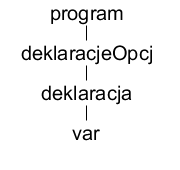
\includegraphics[scale=0.5,bb=0 0 180 170]{grafika/prosteDrzewo/program_deklaracjeOpcj_deklaracja_VAR.png}
   \caption{Pierwszy terminal VAR}
\end{figure}

Myślę że sam algorytm zaczyna się już klarować. Dlatego pominę dalszy rozwój \verb|deklaracja| i przejdźmy do chwili jej zakończenia. Rysuję drzewo rozbioru
\begin{figure}[htb] %rzucilo na dol strony
   \centering
   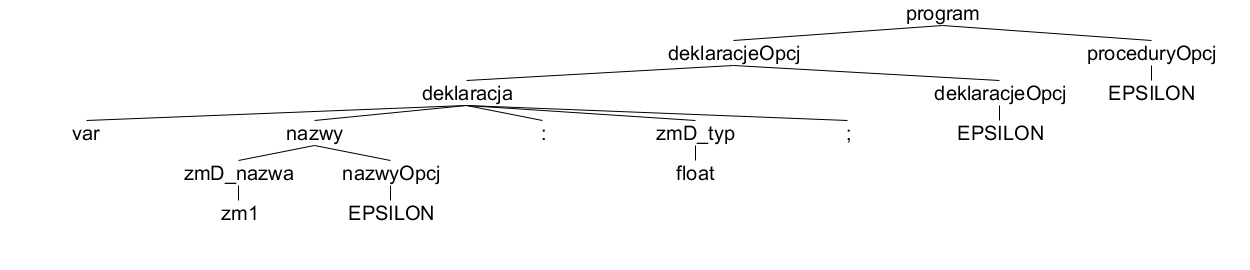
\includegraphics[scale=0.5,bb=0 0 1250 270]{grafika/prosteDrzewo/program_start.png}
   \caption{Moment zamknięcia deklaracji}
\end{figure}
\newpage
oraz załączam zrzut stosu
\begin{verbatim}
@stosy = (
  [],
  [ 'proceduryOpcj' 'START' 'instrukcje' 'END' ],
  [ 'deklaracjeOpcj' ],
  );
\end{verbatim}
Prawie Dajavu z drugiego poziomu, zniknęła tylko rozpracowana właśnie \verb|deklaracja|. Znów napotykamy \verb|deklaracjeOpcj|, które, jeśli zadeklarowalibyśmy następną zmienną, ponownie pozostawią na stosie [ \verb|deklaracja|, \verb|deklaracjaOpcj| ] i po rozłożeniu których znowu zastalibyśmy stos w stanie przedstawionym wyżej. Jednakże nic już nie deklarujemy, a badany obecnie leksem jest klasy terminalowej \verb|START|. Parsing dla takich argumentów oddaje \verb|EPSILON|. Cechą terminali jest, że ich gramatyka oddaje siebie samych. Tak więc
\begin{verbatim}
@stosy = (
  [],
  [ 'proceduryOpcj' 'START' 'instrukcje' 'END' ],
  [ 'EPSILON' ],
  );
\end{verbatim}
Po zawieszeniu na drzewie \verb|EPSILON| najwyższy stos będzie pusty. W takiej sytuacji cofamy się na drzewie rozbioru do przodka. \verb|proceduryOpcj| podłączane są do symbolu pierwotnego \verb|program|, do nich \verb|EPSILON|. \verb|START| występuje w leksemie, \verb|instrukcje| są puste i \verb|END| kończy kod źródłowy. Zastając puste stosy, analiza zostaje zakończona z rezultatem:
\begin{figure}[h!]
   \centering
   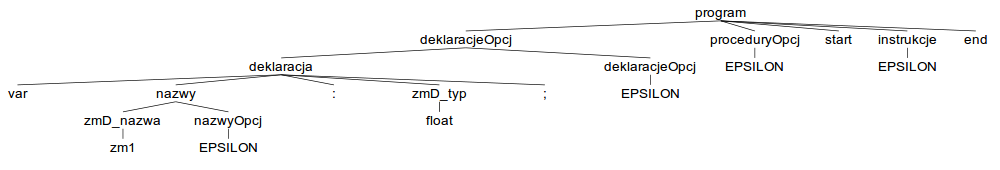
\includegraphics[scale=0.5,bb=0 0 1000 170]{grafika/prosteDrzewo/prosteDrzewoFinal.png}
   \caption{Rozbiór kodu źródłowego}
\end{figure}

\newpage
\lstinputlisting[label=Kompilator::Pascal::Syntaktyka,caption=główna część metody analizuj z klasy Kompilator::Pascal::Syntaktyka]{zrodla/syntaktyka_analizuj.pl}

\newpage
\subsection{Semantyka}
Docierając do tego etapu dysponujemy poprawnym pod kątem syntaktycznym drzewem rozbioru. Teraz należy wyodrębnić padające deklaracje nazw własnych i je zapamiętywać wraz z ich kontekstem. W przypadku późniejszego odwołania do takowych sprawdzamy czy nazwa jest nam znana i wyrzucamy błąd, jeśli nie jest.

Semantyka jest zbiorem reguł ograniczających swawolę programisty, jednocześnie gwarantujących przewidywalność działania programu.
\subsubsection{Wymagania}
Nie mogą istnieć deklaracje zmiennych o tych samych nazwach na tym samym poziomie. Na różnych są dopuszczalne, wtedy deklarowane póżniej przesłaniają wcześniejsze, do których tracimy dostęp.

Wyróżniamy trzy rodzaje wartości: wartości stałe oraz zapisane w zmiennych globalnych i lokalnych. Typ może być prosty: literał znakowy, liczba całkowita, zmiennoprzecinkowa, wartość logiczna; lub być typem tablicowym, czyli zawierać zestaw typów prostych. W takim wypadku przed użyciem należy zaalokować dla niego miejsce i nie wykraczać poza nie. Nie można drugi raz alokować miejsca dla zmiennej już zaalokowanej, nie można dwa razy tego samego miejsca zwolnić. Zapamiętywane własności operandu stanowią jego maskę.

W definicjach funkcji wolno wywoływać funkcje, których deklaracja nie jest jeszcze znana, a nastąpi w dalszej części pliku. Wymusza to dwuprzebiegowy proces analizy - wstępny zapamięta wszystkie deklaracje funkcji (wraz z maskami przyjmowanych argumentów), kolejny zajmie się właściwą pracą.

Wywołania funkcji można zagnieżdżać. Oznacza to, że wywołując funkcję można jako argumenty stosować wyrażenie i przekazywać jego końcowy wynik. A w skład wyrażenia może wychodzić wywołanie kolejnej funkcji również ze zbiorem wyrażeń w argumentach.

Dla procesu syntezy stracą znaczenie nazwy zmiennych i procedur, ważny stanie się przyporządkowany im numer i maska. Dlatego nazwy własne pozostaną w obszarze semantyki, która pozostawi je sobie samej.

% todo Operatory jedno dwuragrumentowe tutaj

\begin{table}[h!]
\centering

\begin{minipage}{5.5cm}
\centering
\begin{tabular}{|r|l|}
  \hline 
  1dd & stała\\
  \hline
  2dd & zmienna globalna \\
  \hline
  3dd & zmienna lokalna \\
  \hline
\end{tabular} 
\caption{Rodzaje wartości}
\end{minipage}
\begin{minipage}{5.5cm}
\centering
\begin{tabular}{|r|l|}
  \hline 
  d0d & typ prosty\\
  \hline
  d1d & typ złożony, niezaalokowany \\
  \hline
  d2d & typ złożony, zaalokowany \\
  \hline
\end{tabular} 
\caption{Tablice}
\end{minipage}
\begin{minipage}{5.5cm}
\centering
\begin{tabular}{|r|l|}
  \hline 
  dd1 & integer\\
  \hline
  dd2 & float \\
  \hline
  dd3 & boolean \\
  \hline
  dd4 & string \\
  \hline
\end{tabular} 
\caption{Typy wartości}
\end{minipage}

\caption{Rozkład masek operandów}
\end{table}


\subsubsection{Opis języka}
Pod uwagę brane są linie zawierające piąty separator. Po nim następuje wyrażenie stanowiące pełnioną przez klasę funkcję. Para nazwa klasy i funkcja jest opisem semantyki. Funkcje:
%\begin{table}[h!]
%\centering
%\begin{tabular}{|l|l|}

\setlongtables
\begin{longtable}{|l|l|} % * \textwidth
%\hline
%Gałąź & Znaczenie \\
%\endfirsthead
%\endlastfoot
  \hline 
  procedura & Znacznik informuje o wejściu do ciała procedury\\
  \hline
  prD\verb|_|nazwa & Następująca nazwa własna będzie nazwą analizowanej właśnie procedury\\
  \hline
  prD\verb|_|typ & Następujący typ będzie typem analizowanej właśnie procedury \\
  \hline
  parametryOpcj & Następują deklaracje parametrów procedury\\
  \hline
  parametr & Następuje deklaracja parametru procedury\\
  \hline
  deklaracja & Deklarowana będzie zmienna lub parametr procedury\\
  \hline
  zmD\verb|_|nazwa & Następująca nazwa własna będzie nazwą deklarowanej zmiennej\\
  \hline
  zmD\verb|_|typ & Następujący typ będzie typem deklarowanej zmiennej\\
  \hline
  prW\verb|_|nazwa & Następująca nazwa własna będzie nazwą wywoływanej procedury\\
  \hline
  pmW & Następuje przekazywanie argumentu do wywoływanej procedury\\
  \hline
  zmW\verb|_|nazwa & Następująca nazwa własna będzie nazwą wywoływanej zmiennej\\
  \hline
  zmA\verb|_|nazwa & Następująca nazwa własna będzie nazwą zmiennej alokowanej\\
  \hline
  zmZ\verb|_|nazwa & Następująca nazwa własna będzie nazwą zmiennej zwalnianej\\
  \hline
  alokacjaD & Znacznik informuje o alokacji pamięci\\
  \hline
  zwolnienieD & Znacznik informuje o zwalnianiu zajętej pamięci\\
  \hline
  liczbaint & Analizowany typ jest liczbą całkowitą\\
  \hline
  liczbaf & Analizowany typ jest liczbą zmiennoprzecinkową\\
  \hline
  logika & Analizowany typ jest wartością logiczną\\
  \hline
  lznakowy & Analizowany typ jest literałem znakowym\\
  \hline
  arrayof & Analizowany typ jest złożony\\
  \hline
  lubwyrazenie & Znacznik informuję o następującym nowym wyrażeniu\\
  \hline
  przypisanieD & Znacznik informuje o mającym nastąpić przypisaniu wartości do zmiennej\\
  \hline
  plusm1 & Następujący operator jest jednoargumentowym +-\\
  \hline
  plusm & \multirow{9}{*}{Następujący operator dwuargumentowy} \\
  razyd & \\
  zaleznosc & \\
  and & \\
  or & \\
  rowne & \\
  nawoo & \\
  nawoz & \\
  naklz & \\
  \hline
  blokD & Deklaracja bloku. Wewnątrzne deklaracje zmiennych przesłonią obowiązujące\\
  \hline
  zwrot & Następuje powrót z procedury\\
  \hline
%\hline
%\caption{Gałęzie funkcyjne} \label{tab:tags}\\
\end{longtable}

\subsubsection{Logika}
Działanie polega na rekursywnym przejściu przez drzewo rozbioru i śledzeniu aktywności gałęzi funkcyjnych. Dotarłszy do znaczącego terminatora sprawdzamy ustawienia zworek aktywności i w zależności od ich położeń wykonujemy akcje na obiekcie syntezy.

Funkcja \verb|_|szukajFunkcji zbada tym sposobem definicje procedur - zapamięta maski parametrów oraz nazwę i typ samej procedury. Jest to analiza wstępna. 

\lstinputlisting[label=Kompilator::Pascal::Semantyka,caption=metoda szukajFunkcji z klasy Kompilator::Pascal::Semantyka]{zrodla/semantyka_szukajFunkcji.pl}

Po tym nastąpi właściwa analiza wywołań zmiennych i fukcji w metodzie \verb|_|sprawdzWywolania. Schemat jej działania jest bardzo podobny.

\begin{wrapfigure}{r}{0.5\textwidth}
  \begin{center}
    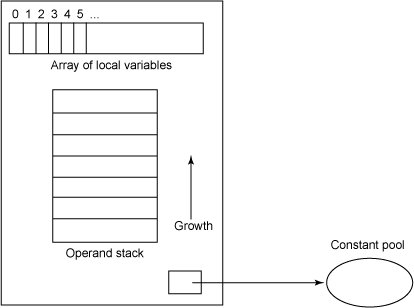
\includegraphics[scale=0.5,width=0.48\textwidth]{grafika/vm.png}
  \end{center}
  \caption{Ramka}
\end{wrapfigure}

\subsection{Synteza}
\subsubsection{JVM}
Wirtualna maszyna Javy jest maszyną stosową. Każdy wykonywany wątek ma swój osobny stos tzw. ramek. Wywołując metodę, odkładamy na stos nową ramkę. Składa się ona z referencji do pól statycznych klasy wywoływanej metody, tablicy parametrów lokalnych o znanej wielkości (policzonej na etapie kompilacji metody) oraz stosu operandów. Jeśli metoda jest wirtualna, pierwszym parametrem lokalnym jest referencja do \verb|this|.

Wykonywana metoda działa wg schematu zapisanego we własnym kodzie bajtowym. Może ładować swoje parametry na stos, tam konwertować ich typy, wykonywać obliczenia i zapisywać wynik znowu w parametrach lokalnych. W trakcie działania wywołuje inne metody, wtedy nowa ramka przesłani chwilowo obecną. Po powrocie na stosie bieżącej ramki zastaniemy ewentualny zwrócony operand.

Dane na stosach operandów mają podstawową szerokość 32 bitów. Ładując typ mniejszy, jest on rozszerzany, operując \verb|long|-iem wykorzystujemy dwa słowa.

\subsubsection{ONP}
Odwrotna Notacja Polska jest sposobem zapisu wyrażeń matematycznych. Opracował ją Charles Homblin opierając się na Notacji Polskiej Jana Łukasiewicza i ją "odwracając". Zapis
\begin{verbatim}
2 + 3 * 4 - 5
\end{verbatim}
W ONP wygląda
\begin{verbatim}
2 3 4 * + 5 -
\end{verbatim}
Do obliczenie wartości wyrażenia pobiera się kolejne symbole z ciągu i w razie napotkania operatora wylicza się nim dwie ostatnie wartości i na ich miejsce wstawiany jest wynik. Kolejne kroki
\begin{verbatim}
2 3 4 * + 5 -
2 12 + 5 -
14 5 -
9
\end{verbatim}
Czemu to służy? Procesor RISC w jednej instrukcji może obliczać dwie wartości ulokowane w dwóch rejestrach, co przenosi się na JVM, która w jednym opkodzie może obliczać dwie wartości ze szczytu stosu. Dlatego złożone wyrażenia należy rozbić na zestaw prostych instrukcji dwuargumentowych. Rozpracowując takie wyrażenie w naturalnym zapisie musimy uważać na priorytety operatorów tzn. wstrzymać się z obliczeniami do momentu uzyskania wyniku operandów o wyższym priorytecie. ONP znakomicie rozstrzyga problem margnizując priorytety w określaniu kolejności operacji.

\subsubsection{Kod bajtowy}
Spójrzmy na przykładowe opkody
\setlongtables
\begin{longtable}{|l|l|l|l|l|} % * \textwidth
\hline
Mnemonik & Opkod & Dod. bajty & stos operandów & opis \\
%\endfirsthead
%\endlastfoot
  \hline
  iconst\verb|_|m1 & 02 &  & -> -1 & ładuje stała -1 jako int\\
  \hline
  iconst\verb|_|0 & 03 &  & -> 0 & ładuje stała 0 jako int\\
  \hline
  fconst\verb|_|1 & 0b &  & -> 0.0f & ładuje stałą -1.0 jako float\\
  \hline
  ldc & 12 & idx & -> w & ładuje stałą o indeksie \verb|idx|\\
  \hline
  iload & 15 & idx & -> w & ładuje parametr \verb|idx| jako int\\
  \hline
  iload\verb|_|0 & 1a &  & -> w & ładuje parametr 0 jako int\\
  \hline
  fload\verb|_|1 & 23 & idx & -> w & ładuje parametr 1 jako float\\
  \hline
  istore & 36 & i & w -> & wrzuca wartość inta do parametru \verb|i|\\
  \hline
  iastore & 4f &  & ref idx w -> & wrzuca wartość inta \verb|w| do tablicy \verb|ref| pod \verb|idx|\\
  \hline
  aastore & 53 &  & ref1 i ref2 -> & wrzuca referencję \verb|ref2| do tablicy \verb|ref1| pod \verb|i|\\
  \hline
  getfield & b4 & idx1, idx2 & ref -> w & ładuje pole \verb|idx1<<8+idx2| obiektu ref\\
  \hline
  putfield & b5 & idx1, idx2 & ref w ->  & zapisuje pole \verb|idx1<<8+idx2| obiektu ref\\
  \hline
  anewarray & b5 & i1, i2 & r -> ref & nowa tablica klasy \verb|i1<<8+i2| o rozmiarze \verb|r|\\
  \hline
  l2i & 88 &  & w -> wynik & rzutowanie long na int\\
  \hline
  i2f & 86 &  & w -> wynik & konwersja int do float\\
  \hline
  fadd & 62 &  & w1, w2 -> wynik & dodaje 2 ostanie liczby jako float\\
  \hline
  iand & 7e &  & w1, w2 -> wynik & logiczny and między 2 intami\\
  \hline
  fneg & 76 &  & w -> wynik & neguje floata\\
  \hline
  if\verb|_|acmpeq & a5 & b1 b2 & ref1 ref2 -> & skok o \verb|b1<<8+b2| jeśli referencje się zgadzają\\
  \hline
  if\verb|_|icmplt & a1 & b1 b2 & w1 w2 -> & skok o \verb|b1<<8+b2| jeśli \verb|w1| mniejsze od \verb|w2|\\
  \hline
  goto & a7 & b1 b2 & -> & skok o \verb|b1<<8+b2|\\
  \hline
  ireturn & ac &  & w -> [pusty] & zwraca inta z metody\\
  \hline
  invSpec & b7 & i1, i2 & ref, [arg] -> w & wywołuje metodę \verb|i1<<8+i2| obiektu ref z \verb|arg|\\
  \hline
  instOf & c1 & i1, i2 & ref, -> w & sprawdza czy \verb|ref| jest klasy \verb|i1<<8+i2|\\
  \hline
  athrow & bf & i1, i2 & ref -> [pusty] ref & rzuca wyjątek \verb|ref|, czyści stos \\
  \hline  
\caption{Wybrane opkody} \label{tab:tags}\\
\end{longtable}

Mnemoniczny jednoliterowy przedrostek uwidacznia typ prymitywny na którym opkod operuje. 

Wszystkie opkody zapisane są w jednym bajcie. Pewne z nich wymagają dodatkowych bajtów następujących w strumieniu kodu pośredniego. Opkod \verb|iload| załaduje na stos wartość parametru ramki znajdującego się pod indeksem określonym w następnym bajcie. Istnieją skrócone opkody np zawierające już indeks parametru jak \verb|iload_0|.

Pewne opkody odwołują się do metod lub pól klasy poprzez numer indeksowy zapisany w strumieniu. Wyraża on faktyczne nazwy - przyporządkowanie zapisane jest w plikach .class.

\newpage
\begin{table}[h!]
\centering

\begin{minipage}{8cm}
\centering
\begin{verbatim}
$ cat A.java
class A {








  void a() {
    int zm1 = 3;
  }
  
  
  
  long b(long zm1, float zm2) {
    int zm3 = -1;
    zm2 = zm1 + zm3 * (8 - 2);
    return zm1;
  }









}
\end{verbatim}
\end{minipage}
\begin{minipage}{8cm}
\centering
\begin{verbatim}
$ javap -c A
Compiled from "A.java"
class A extends java.lang.Object{
A();
  Code:
   0:	aload_0
   1:	invokespecial	#1; //Method java/lang/Object."<init>":()V
   4:	return

void a();
  Code:
   0:	iconst_3
   1:	istore_1
   2:	return

long b(long, float);
  Code:
   0:	iconst_m1
   1:	istore	4
   3:	lload_1
   4:	iload	4
   6:	bipush	6
   8:	imul
   9:	i2l
   10:	ladd
   11:	l2f
   12:	fstore_3
   13:	lload_1
   14:	lreturn
}
\end{verbatim}
\end{minipage}

\caption{Porównanie Javy i jej bajtkodu}
\end{table}



\subsubsection{Konkretyzacja}
Zadaniem kompilatora jest generowanie dowolnego bajtkodu poprzez zaimplementowanie pod jego kątem klasy abstrakcyjnej. Aby spełniał walory użytkowe konkretyzacja musi być prosta. Klasa abstrakcyjna:
\lstinputlisting[label=Kompilator::Api::Synteza::Class,caption=klasa abstrakcyjna Kompilator::Api::Synteza::Class]{zrodla/class.pm}
\newpage
Javowa konkretyzacja:
\lstinputlisting[label=Kompilator::Java::Synteza::Class,caption=fragment Kompilator::Java::Synteza::Class]{zrodla/classLight.pl}

\section{Projekt}

\subsection{Budowa}
Projekt zbudowany jest jako moduł przy wykorzystaniu narzędzia Module::Starter dostępnego w bibliotece cpan \footnote{instalacje w unixach jako root: cpan -i Wybrany::Modul}. Szkielet modułu zawiera plik Makefile.PL, który po uruchomieniu tworzy właściwy Makefile. Mamy w nim dostępne cele takie jak make, make test, make install, make clean. Nie mając uprawnień super użytkownika, nie uda się makefilem modułu osadzić w systemie, czyli przekopiować plików do ścieżek wymienionych w @INCLUDE
\begin{verbatim}
perl -e "print qq(@INC)"
\end{verbatim}
Inne wykorzystane moduły
\begin{description}
	\item[constant]: Deklaracje stałych
	\item[strict]: Wymusza bardziej restrykcyjne zachowanie VM
	\item[warnings]: Drukuje ostrzeżenia
	\item[warnings::register]: Warunkowe ostrzeżenia
	\item[Carp]: Drukuje diagnostyke lub przerywa program
	\item[module "switch"]: Konstrukcja "switch"
	\item[XML::DOM]: Dostęp DOM do drzewa XML
	\item[Data::Dumper]: Zrzuty struktur
	\item[Aspect]: Aspektowy paradygm programowania
	\item[FindBin]: Lokalizacja skryptu
	\item[lib]: Ścieżki wyszukiwań modułów
	\item[Test::More]: Testy
	\item[Test::Exception]: Testy wyjątków
\end{description}

\newpage
\subsection{Model}

\subsubsection{Klasy}

\begin{figure}[h!]
   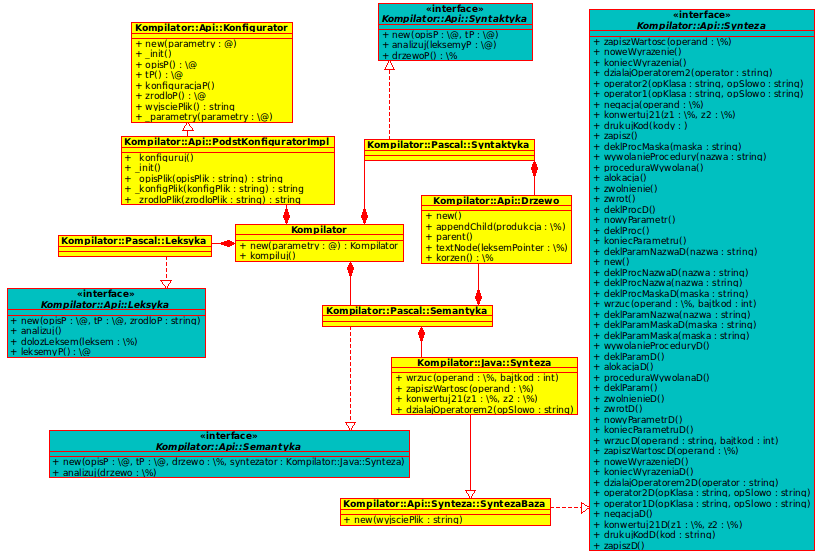
\includegraphics[width=15cm]{grafika/model/rdzen.png}
   \caption{Rdzeń analiz}
\end{figure}

\begin{description}
	\item[Kompilator]: buduje świat i rozpoczyna analizy
	\item[Kompilator::Api::Konfigurator]: Baza dla zaimplementowania konfiguracji działania kompilatora
	\item[Kompilator::Api::PodstKonfiguratorImpl]: Czyta podstawowe pliki wejściowe, ustanawia konfigurację
	\item[Kompilator::Pascal::Leksyka]: Odpowiada za analizę leksykalną.
	\item[Kompilator::Pascal::Syntaktyka]: Odpowiada za budowę drzewa rozbioru.
	\item[Kompilator::Api::Drzewo]: Struktura drzewa rozbioru.
	\item[Kompilator::Pascal::Semantyka]: Implementuje dwuprzebiegową analizę semantyczną.
	\item[Kompilator::Api::Synteza]: Interfejs wywołań zwrotnych.
	\item[Kompilator::Api::Synteza::SyntezaBaza]: Szkielet do syntezy kodu bajtowego. Deleguje wywołania zwrotne do klas specjalistycznych.
	\item[Kompilator::Java::Synteza]: Dziedziczy po SyntezaBaza, może wpłynąć na zachowanie przodka.
\end{description}

Uproszczenie konkretyzacji wyjściowych bajtkodów jest zrealizowane poprzez zestaw klas
\begin{figure}[h!]
   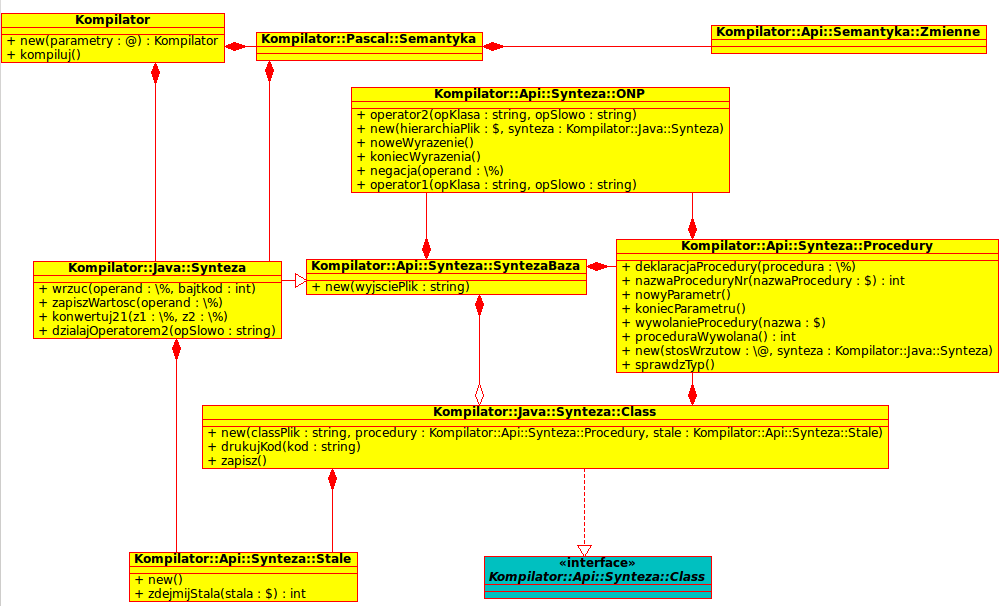
\includegraphics[width=15cm]{grafika/model/end2.png}
   \caption{End}
\end{figure}
\begin{description}
	\item[Kompilator]: buduje świat i rozpoczyna analizy
	\item[Kompilator::Pascal::Semantyka]: Implementuje dwuprzebiegową analizę semantyczną.
	\item[Kompilator::Api::Semantyka::Zmienne]: Klasa pomocnicza, opiekuje się nazwami zmiennych, przeprowadza deklaracje, sprawdza wywołania. Przechowuje tablicę globalną zmiennych oraz stos lokalnych. Zajmuje się maskowaniem alokacji i dealokacji.
	\item[Kompilator::Api::Synteza::SyntezaBaza]: Deleguje aktywność gałęzi funkcjonalnych na specjalizowane klasy pomocnicze.
	\item[Kompilator::Api::Synteza::ONP]: Przetwarza złożone wyrażenia do trójwersowych. Buduje do tego stosy zmiennych i operatorów. 
	\item[Kompilator::Api::Synteza::Procedury]: Przechowuje padające definicje procedur, buduje stos wywołań funkcji. Konwertuje typy wywoływanych argumentów. Wyrzuca błąd jeśli wywołana argumentów nie zgadza się ze zdefiniowaną. Potrzebuje referencji onp w celu obsługi złożonych wyrażeń w wywołaniach.
	\item[Kompilator::Java::Synteza]: Dziedziczy po SyntezaBaza, może wpłynąć na zachowanie przodka. Operuje maskami w celu wydelegowania właściwego opkodu.
	\item[Kompilator::Api::Synteza::Class]: Interfejs do implementacji dla konkretnych bajtkodów.
	\item[Kompilator::Java::Synteza::Class]: Właściwa konkretyzacja produkowanego bajtkodu.
\end{description}

Aspektowo zorienowane logowanie działań poszczególnych etapów
\begin{figure}[h!]
   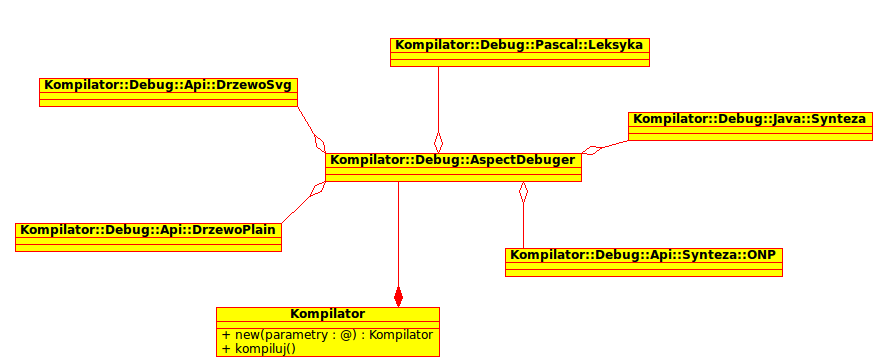
\includegraphics[width=15cm]{grafika/model/end.png}
   \caption{Logowanie}
\end{figure}

\begin{description}
	\item[Kompilator::Debug::AspectDebugger]: Rdzeń logowania aspektowego. Na podstwie otrzymanej konfiguracji tworzy obiekty logowań i uruchamia aspekty.
	\item[Kompilator::Debug::Pascal::Leksyka]: Wypisuje przyjętą klasyfikację oraz rozpoznany zbiór leksemów
	\item[Kompilator::Debug::Api::DrzewoPlain]: Wypisuje strukturę drzewa rozbioru syntaktycznego w czystej formie tekstowej
	\item[Kompilator::Debug::Api::DrzewoSvg]: Buduje strukturę drzewa w pliku XML korzystając z szablonu http://weston.ruter.net/projects/syntax-tree-drawer/
	\item[Kompilator::Debug::Java::Synteza]: Drukuje wywołania funkcji wraz z przyjętymi argumentami dla klas z nazwą Kompilator::Java::Synteza::
	\item[Kompilator::Debug::Java::Synteza]: Drukuje wywołania funkcji wraz z przyjętymi argumentami dla klas z nazwą Kompilator::Java::Synteza::
	\item[Kompilator::Debug::Api::Synteza::ONP]: Informuje o działaniach na stosie ONP
\end{description}

\newpage
\subsubsection{Sekwencje}
\begin{figure}[h!]
   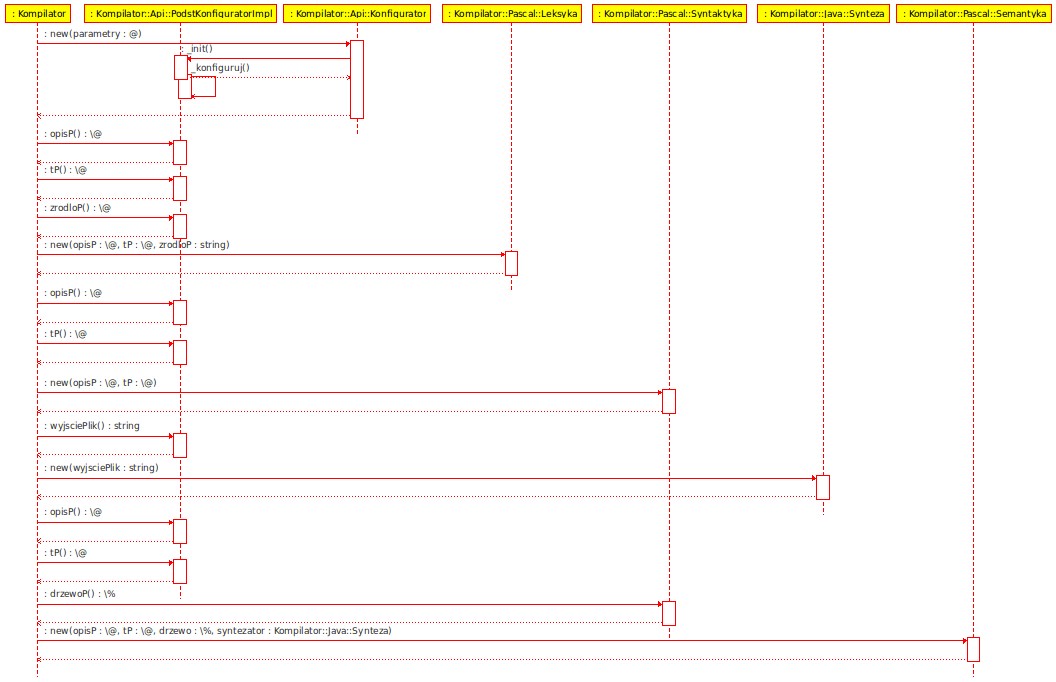
\includegraphics[width=15cm]{grafika/model/rozruch.png}
   \caption{Budowa świata}
\end{figure}

\begin{figure}[h!]
   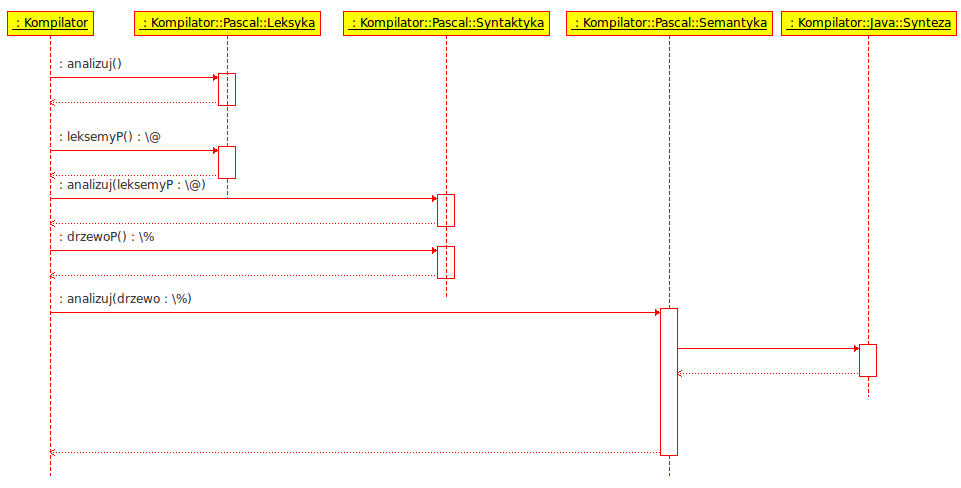
\includegraphics[width=15cm]{grafika/model/analizy.png}
   \caption{Kompilacja}
\end{figure}

\newpage
\subsection{Zastosowanie}
Skompilujmy kod źródłowy
\lstinputlisting[label=zrodla:in.pas,caption=Przykładowy kod źródłowy]{zrodla/in.pas}
Wynik uzupełniony o komentarz
\begin{verbatim}
$ perl Kompilator.pl zrodloPlik=/zrodla/in.pas
SuccesFull
real	0m4.685s # Intel Atom N270
user	0m4.600s # Ubuntu 10.04 Lucid Lynx
sys	0m0.064s     # 2.6.32-28-generic
$ cat A.class 

# cialo procedury liniowa
ldc 0 # laduje pierwsza stala 4, bedzie intem
ldc 1 # laduje druga stala 3.5, bedzie floatem
iload 0 # laduje przekazany parametr jako int
i2f # konwertuje parametr na float
fmul # mnozy szczytowe liczby zmiennoprzecinkowe
f2i # wynik konwertuje do inta
iadd # dodaje 2 szczytowe inty
# brakuje return


# cialo procedury funkcja
iload 2 # laduje wartosc z trzeciego parametru, zm3 int
ldc 2 # laduje trzecia stala 2, bedzie intem
fload 0 # laduje pierwszy parametr, zm1 float
f2i # konwertuje wartosc parametru na int
imul # mnozy inty ze szczytu 2 * zm1
ldc 3 # laduje czwarta stala 3, typ calkowity
iload 1 # laduje drugi parametr, zm2 int
imul # mnozy inty ze szczytu 3 * zm2
iadd # dodaje wyniki obu mnozen
istore 2 # zapisuje wynik pod trzecia zmienna zm3 jako int

fload 0 # laduje pierwszy parametr zm1 jako float
ldc 4 # laduje piata stala 5, bedzie intem
invoke 0 # wywoluje procedure liniowa
i2f # wynik wywolania konwertuje na float
fstore 0 # zapisuje go w zm1

fload 0 # laduje zm1 jako float
iload 1 # laduje zm2 jako int
iload 2 # laduje zm3 jako int
iadd # dodaje inty zm2 + zm3
i2f # wynik konwertuje na float
fadd # dodaje floaty zm1 + (zm2+zm3)
#brakuje return


# wnetrze glownej czesci programu
getfield 0 # laduje zmienna globalna zm1, int
# blad powinien zaladowc parametr lokalny 0, ktory powinien byc referencja this
ldc 3 # laduje czwarta stala calkowita 3
ldc 0 # laduje pierwsza stala calkowita 4
imul # mnozy stale
putfield 0 # wynik zapisuje w zmiennej globalnej zm1
getfield 1 # laduje zmienna globalna zm2, int
ldc 2 # laduje trzecia stala 2, int
getfield 0 # laduje pierwsza zmienna globalna zm1, int
iadd # dodaje 2+zm1
invoke 0 # wywoluje pierwsza funkcje zagniezdzona, liniowa
ldc 0 # laduje pierwsza stala 4, int
invoke 1 # wywoluje druga funkcje zewnetrzna, funkcja
\end{verbatim}
Na pewno brakuje instrukcji powrotów z funkcji. Niewłaściwie traktowane jest przypisanie wartości do pól klasy. Kompilator powinien ściągnąc z tablicy lokalnej argument 0, który powinien być referencją na "ten" obiekt. Parametry procedur powinny zaczynać się od pierwszego indeksu. ONP działa poprawnie, zagnieżdżone wywołania funkcji również.

Do zaimplementowania pozostają przede wszystkim instrukcje skoku goto. Od miejsc rozgałęzień w kodzie źródłowym należy zliczać produkowane bajty strumienia pośredniego do ponownego zejścia alternatywnych dróg. Ilość bajtów zapisać po ifie w strumieniu jako offset. Do tego zadania należałoby wyodrębić odrębną klasę jako pomocniczą dla Kompilator::Api::Semantyka::SemantykaBaza.

Brakuje wydruku opkodów obsługi tablic. Atutem jest, iż klasa Kompilator::Pascal::Semantyka nie pozwala przydzielić pamięci do zmiennej zaalokowanej oraz zwolnić nieprzydzieloną.

Ułatwieniem byłaby obsługa nawiasowania w wyrażeniach, Kompilator::Api::Semantyka::Zmienne są na taką okoliczność przygotowane. Wystarczy uwzględnić je w zewnętrznym pliku opisu języka.


Repozytorium projektu:
\begin{center}
	\fbox{\texttt{git://krystianwojtas.eu/kompilator}}
\end{center}


\newpage
\section{bibliografia}
\begin{description}
	\item \verb|http://home.agh.edu.pl/~marcino/Uczelnia/Files/JFA/zajecia03JFA.pdf|
	\item \verb|http://home.agh.edu.pl/~tekomp/pages/referaty/referaty-studenckie/5-1.htm|
	\item \verb|http://pl.wikipedia.org/wiki/Analiza_sk%C5%82adniowa|
	\item \verb|http://pl.wikipedia.org/wiki/Parser_LR|
	\item \verb|http://www.ibm.com/developerworks/ibm/library/it-haggar_bytecode/|
	\item \verb|http://en.wikipedia.org/wiki/Java_bytecode_instruction_listings|
	\item \verb|http://en.wikipedia.org/wiki/Class_%28file_format%29|
	\item \verb|http://java.sun.com/docs/books/jvms/second_edition/html/ClassFile.doc.html|
	\item \verb|http://www.tutorialspoint.com/perl/perl_oo_perl.htm|
	\item \verb|http://weston.ruter.net/projects/syntax-tree-drawer/|
	\item \verb|http://onjava.com/pub/a/onjava/2004/01/14/aop.html|
\end{description}

\end{document}

